\documentclass[12pt]{report}

\usepackage[T1]{fontenc}
\usepackage[utf8]{inputenc}
\usepackage{graphicx}

\begin{document}
\title{\textbf{Caracteristica de los convertidores de potencia CA-CD, CD-CA, CA-CA y CD-CD\\}}
\author{Enesto Alonso Partida López\\ Universidad Politecnica De La Zona Metropolitana De Guadalajara\\}
\date{17 de septiembre 2019 }
\maketitle

\newpage
{\huge \textbf{Convertidores de CA-CD}\\}
 
 \begin{itemize}
 \item {\Large No controlados}
 \item {\Large Controlados}
 \end{itemize}
 
{\huge\textbf{Convertidores de CD-CA}\\}

 \begin{itemize}
 \item {\Large Por alimentación}
 \item {\Large Por número de fases}
 \item{\Large Por topología}
 \item{\Large Por disposición de carga}
 \item{\Large Por su forma de onda de la salida}
 \end{itemize}
 
{\huge \textbf{Convertidores de CD-CD}\\}
 
 \begin{itemize}
 \item {\Large Recluctor (Buck)}
 \item {\Large Elevador (Boost}
 \end{itemize}
 
 {\huge \textbf{Convertidores de CA-CA}\\}
 
 \begin{itemize}
 \item {\Large Variadores de CA}
 \item {\Large Ciclo controlados}
 \item {\Large Convertidores matriciales}
 \end{itemize}
 
 \newpage
 
 {\huge \textbf{Convertidores de CA-CD}\\}\\
 {\Large Controlados}\\
 
El primer circuito de CA-CD es el que se encuentra formado por tiristores los cuales al forman un puente de diodos, dicho puente tiene la función de convertir la corriente alterna en corriente directa, esto mediante la posición que tienen los tiristores, en dicho circuito siempre se tendrán dos salidas, una positiva y otra negativa, esto sin importar el cambio que tiene el voltaje. Los tiristores funcionan de tal manera que cuando la onda de corriente cambie sus polos estos impidan que la corriente siga su camino y en cambio estos le dan siempre una sola dirección tanto a la carga positiva como a la negativa.\\
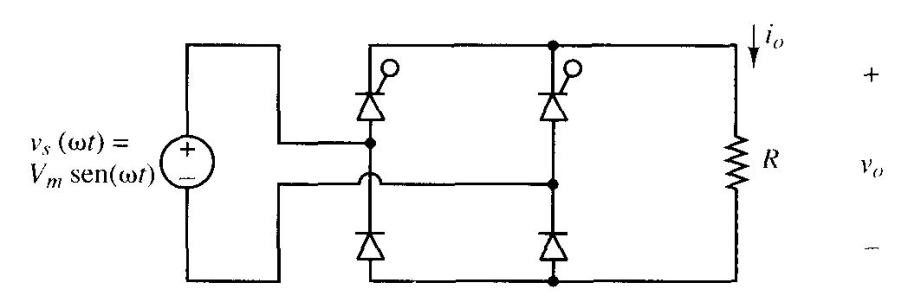
\includegraphics[width=12cm]{tiristor.jpg} 
 
 
 
 A su vez existe la rectificación de media onda, la cual puede ser controlada mediante tiristores, dichos componentes impiden el paso de la corriente negativa o positiva según sea el caso, en cambio colocados en una posición especifica los tiristores tienen la función de evitar  el paso de la corriente positiva  y la corriente negativa segun la posicion del diodo y se obtendra una onda muy similar ala que se muestra a continuacion.\\
 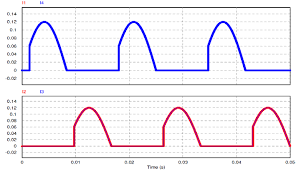
\includegraphics[width=8cm]{images.png} \\
 \newpage
 Por otro lado existe la rectificacion completa en la cual se utiliza un puente de diodos en este caso por ser controlado se utilizan tiristores los cuales impiden el paso de la corriente y la guian hacia un solo sentido ya sea positivo o negativo, mas estas terminales nunca cambiaran sin importar los ciclos; pero dicho circuito siempre conducirá a la corriente a un mismo punto ya sea positivo o negativo por lo cual al final se tendrá un polo positivo y otro negativo.\\
 \begin{figure}[hbtp]
 \centering
 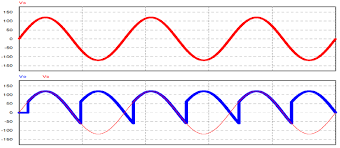
\includegraphics[scale=1]{completa.png}
 \caption{Rectificación de onda completa } 
 \end{figure}\\
 {\huge \textbf{Convertidores de CD-CA}\\}\\
 
  {\Large Topología}\\
 Algunos ejemplos de estos son los MOSFET o bien transistores bipolar de compuerta aislada.\\\\
 
 {\Large Inversores de fuente de voltaje}\\\\
  Estos circuitos se conforman de dos transistores, dos diodos, la fuente y la carga. los transistores permiten que la energía fluya de transmisor a receptor y el diodo en paralelo tiene la misma función, pero en sentido contrario. el funcionamiento del medio puente consiste en que cada transistor actúe durante cada media onda de la señal, esto da como resultado una onda senoidal.\\
  \begin{figure}[hbtp]
  \caption{Inversor de fuente de voltaje}
  \centering
  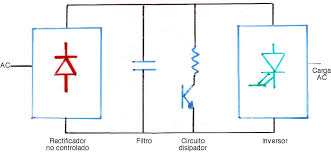
\includegraphics[scale=1]{vsi.jpg}
  \end{figure}
  \\\begin{figure}[hbtp]
  \caption{VSI}
  \centering
  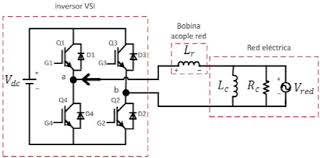
\includegraphics[scale=1]{descarga.jpg}
  \end{figure}
  
{\huge\textbf{Convertidores de CD-CD}\\}\\
 
 {\Large Elevador}\\\\
 Estos circuitos consisten, como su nombre lo dice, subir el voltaje de entrada, esto mediante la utilización de transistores, bobinas y capacitores, principalmente se utiliza un MOSFET para interrumpir la corriente.
Dicho esto, la corriente se elevará al fluir mediante el inductor y el transistor, posteriormente se desconectará el transistor, y cuando se vuelve a activar esta energía saldrá aumentada según sea el capacitor e inductor. 
\\
 \begin{figure}[hbtp]
 \caption{Funcionamiento Elevador}
 \centering
 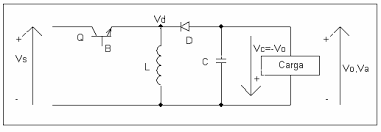
\includegraphics[scale=1]{Elevador.png}
 \end{figure}
 \\{ \Large Convertidor Reductor-Elevador}\\
 \\ En este convertidor es similar al de elevador solo con la diferencia que el voltaje de salida puede ser mayor o menos que el voltaje principal, y la polaridad del voltaje de salida es inverso al voltaje de entrada\\
 \begin{figure}[hbtp]
  \caption{CONVERTIDOR  REDUCTOR-ELEVADOR }
  \centering
  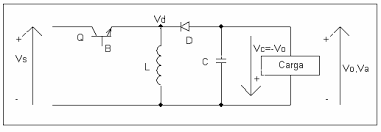
\includegraphics[scale=1]{REDUCTOR-ELEVADOR.png}
  \end{figure}
   
\newpage
 {\huge \textbf{Convertidores de CA-CA}\\}\\
{\Large Control de fase}\\\\
Conocidos también como controlador unidireccional, el cual depende del ángulo de disparo, la potencia que se entregar a la carga solo se podrá controlar en el semiciclo positivo, para dichos circuitos son necesarios tiristores.\\\\
\begin{figure}[hbtp]
\caption{Controll de fase}
\centering
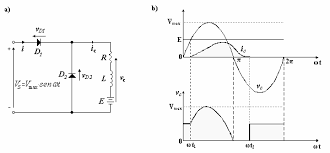
\includegraphics[scale=1]{images (1).png}
\end{figure}

{\Large Controlador monofásico bidireccional }\\

Al igual que el unidireccional, este circuito permite controlar el flujo de la potencia en ambos ciclos ya sea positivo o negativo, la potencia se controladora cambiando el ángulo del tiristor. el desfase entre tiristores será igual a 180 grados .\\\\
\begin{figure}[hbtp]
 \caption{controlador monofasico bidireccional}
 \centering
 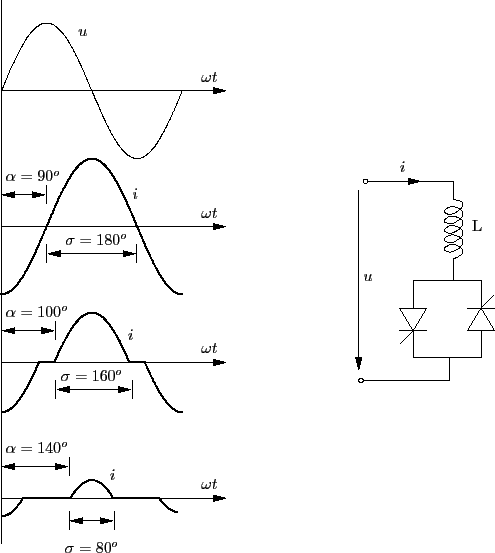
\includegraphics[scale=1]{bidireccional.png}
 \end{figure}
  \newpage
  {\Huge Bibliografías}\\\\
  @thesis{Control de un convertidor de CD-CA monofásico ,
  \author= {Iván Martínez Pérez},
  \title = {Control de un convertidor de CD-CA monofásico},
  type = {Energía de potencia},
  OPTlanguage = {Español},
  OPTpages = {1-66},
  OPTpagetotal = {67},

  }
  

@TechReport{Convertidores CA-CA: controladores de tension alterna y cicloconvertidores,
  author = {anonimo},
  title = {Convertidores CA-CA: controladores de tension alterna y cicloconvertidores},
  institution = {Electronica de potencia},
  year = {2012},
  OPTtype = {reporte},
  OPTnumber = {Ultima edición},
  OPTaddress =Electronica de potencia ,
  OPTmonth = {mayo}
}


  
  

\end{document}